\documentclass{vilniustech}
\vilniustechsetup{
    university={Vilniaus Gedimino technikos universitetas},
    faculty={Fundamentinių mokslų fakultetas},
    cathedral={Informacinių sistemų katedra},
    workTitle={Duomenų atsarginės kopijos/SIEM},
    workType={Namų darbas nr. 4},
    workAuthorGroup={ITSfm-22},
    workAuthorName={Aurimas Šakalys},
    workRecipient={lektorius Vitalijus Gurčinas}
}
\VTDocumentBegin

\section{Duomenų atsraginės kopijos}

\subsection{Programinės įrangos pasirinkimas}

Atsarginėms duomenų kopijoms daryti pasirinkau du įrankius - \textit{borg} ir \textit{Borgmatic}.

\textit{borg} įrankis skirtas daryti atsargines duomenų kopijas. Įrankis veikia \textit{serverio-kliento} principu, kur serveris atlieka duomenų saugojimo užduočių vykdymą, o klientas - deduplikaciją, šifravimą, suspaudimą ir pan. 

\textit{Borgmatic} įrankis skirtas gerokai palengvinti darbą su \textit{borg} atsarginių kopijų darymo įrankiu. Šis įrankis suteikia vartotojui paprastą vartotojo sąsają ir konfiguraciją. Įrankį galima sukonfiguruoti įvariapusiškai, įjungiant ar išjungiant funkcionalumą, kurį suteikia \textit{borg} įrankis.

\subsection{Programinės įrangos diegimas ir konfiguravimas}

Virtualios mašinos kuriamos naudojant \textit{Vagrant} įrankį, o pačios mašinos yra automatiškai sukonfiguruojamos naudojant \textit{Ansible} pjesėmis.

Norint įgyvendinti pirmąjį namų darbo reikalavimą, nusprendžiau atlikti kopijų darymą naudojant \textbf{3-1-2} strategiją. Ši strategija įgyvendinta lokaliai sukuriant dvi virtualias mašinas, į kurias bus talpinamos atsarginės kopijos. Nors praktine prasme abi \textit{borg} serverio virtualios mašinos egzistuoja toje pačioje vietoje, šias virtualias mašinas galima būtų paleisti ir sukonfiguruoti debesų kompiuterijos infrastruktūroje, taip abu atsarginių kopijų serverius patalpinant skirtinguose vietose. Taip \textbf{3-1-2} strategija būtų įgyvendinama praktiškai.

Prieš pradedant atsarginių kopijų sistemos diegimą, klientinėje mašinoje privaloma sugeneruoti SSL raktų porą, kuri bus naudojama autentifikuojantis siunčiant duomenis į atsarginių kopijų serverį. Kiekvieno kliento raktas turi būti įdiegtas į atsarginių kopijų darymo serverius. Diegiant viešajį kliento raktą, šis raktas yra apribojamas \textit{tik} atsarginių kopijų darymo tikslams pridedant šį apribojimą matomą \autoref{lst:restriction}. Tokiu būdu užtikrinama, kad SSL raktų pora negalės būti panaudota kitiems tikslams serveryje. Tolimesni žingsniai apibūdinami tariant, jog tarp serverio ir kliento galima užmegzti saugų SSH ryšį.

\begin{lstlisting}[caption=SSH rakto apribojimas vienai komandai,label={lst:restriction},language=json]
command="borg serve --restrict-to-path /var/local/backups/backup.borg",restrict MIIDDjCCAfY...
\end{lstlisting}

Serverinėse mašinose paprasčiausiai yra įdiegiama \textit{borg} programinė įranga, kuri leis atlikti kopijų darymą klientinei mašinai.

Klientinėje mašinoje, įdiegiami \textit{borg} ir \textit{Borgmatic} įrankiai. \textit{Borgmatic} įrankis yra sukonfiguruojamas naudojant konfiguracinį failą matomą \autoref{lst:borgmatic_config}.

\begin{lstlisting}[caption=\textit{Borgmatic konfiguracija},label={lst:borgmatic_config},language=json]
location:
    source_directories:
        - /home
        - /etc
        - /var/log/syslog*
    repositories:
        - ssh://vagrant@192.168.0.202/var/local/backups/backup.borg
        - ssh://vagrant@192.168.0.203/var/local/backups/backup.borg
        - /var/local/backups/backup.borg

storage:
    encryption_passphrase: "encryption_password"
    ssh_command: ssh -i /home/vagrant/.ssh/id_rsa -o StrictHostKeyChecking=accept-new

retention:
    keep_minutely: 60
    keep_daily: 7
    keep_monthly: 6
    keep_yearly: 1

\end{lstlisting}

Konfiguracija nurodo: 
\begin{itemize}
    \item \textbf{source\_directories} - kurioms direktorijoms/failams norime sudaryti atsarginių duomenų kopijas;
    \begin {itemize}
        \item Šiuo atveju sudarysime direktorijų/failų \textit{/home}, \textit{/etc} ir \textit{/var/log/syslog*} atsargines kopijas.
    \end{itemize}
    \item \textbf{repositories} - į kurias \textit{borg} repozitorijas norėtume talpinti atsargines kopijas;
    \begin {itemize}
        \item Šiuo atveju, dvi atsarginės kopijos talpinamos į du atsarginių kopijų serverius, viena talpinama lokaliai.
    \end{itemize}
    \item \textbf{storage} - nurodo šifravimo slaptažodį ir komandą, naudojamą prisijungti prie atsraginių kopijų serverių;
    \item \textbf{retention} - nurodo kiek, kokio tipo atsarginių kopijų archyvų paliksime. \footnote{Norėčiau atkreipti dėmesį, jog visu 100\% nesuprantu, kokia metodologija yra išlaikomi deduplikuoti duomenys po senų archyvų pašalinimo. \textit{borg} įrankis savo dokumentacijoje šio mechanizmo neaprašo.}
\end{itemize}

Atlikus įrankio konfiguraciją telieka įdiegti \textit{cron} įrašą (\autoref{lst:cron}), kuris kas tam tikrą laiką pakviestų \textit{Borgmatic} įrankį, taip atliekant duomenų kopijų sudarymą ir išsaugojimą.


\begin{lstlisting}[caption={\textit{cron} įrašas, kas minutę kviečiantis \textit{Borgmatic}},label={lst:cron},language=json]
    */1 * * * * root PATH=$PATH:/usr/bin:/usr/local/bin /usr/local/bin/borgmatic --verbosity -1 --syslog-verbosity 1
\end{lstlisting}

\begin{figure}[H]
\begin{center}
    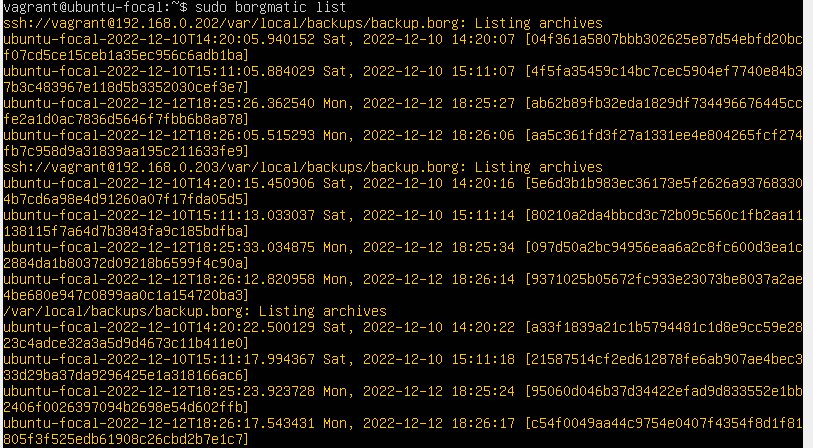
\includegraphics[width=13cm]{img/archives.png}
    \caption{\textit{borg} repozitorijose saugomi archyvai}
    \label{fig:archives}
\end{center}
\end{figure}

\subsection{Užduoties reikalavimų įgyvendinimas}

Atsarginės kopijos atliekamos daromos naudojant \textbf{3-1-2} strategiją, taip įgyvendinant pirmąjį reikalavimą. Kadangi \textit{borg} įrankis yra deduplikuojantis pagal nutylėjimą ir yra padaromos tik pakeistų ar naujų failų atsarginės kopijos, o duomenys yra šifruojami, yra įgyvendinami antras ir penktasis reikalavimai. \textit{borg} įrankis sudaro šifruotas ir inkrementalias atsargines kopijas, taip apsisaugant nuo išpirkos atakų ir įgyvendinant ketvirtą reikalavimą.

Trečiasis reikalavimas įgyvendinamas kiek sudetingiau. Kadangi yra paliekami dienos (septynios), savaitės (keturios) ir mėnesio (šešios) atsarginės kopijos, duomenis galima atkurti naudojant juos, tačiau šie nebūtinai gali vadintis pilnomis atsarginių duomenų kopijomis. Norint pilnai atitikti reikalavimą, kiekvienos savaitės pilnam archyvui tektų sukurti po \textit{borg} repozitoriją. Tai nėra patogu, tačiau tai užtikrintų šimtąprocentinį reikalavimo įgyvendinimą.

Atsarginės duomenų kopijos yra daromos automatiškai, todėl įgyvendinamas ir papildomas reikalavimas.

\section{SIEM}

\subsection{Programinės įrangos pasirinkimas}

SIEM sistemos įgyvendinimui pasirinkau \textit{Wazuh} įrankį dėl paprasto diegimo ir naudojimo. 


\begin{figure}[H]
\begin{center}
    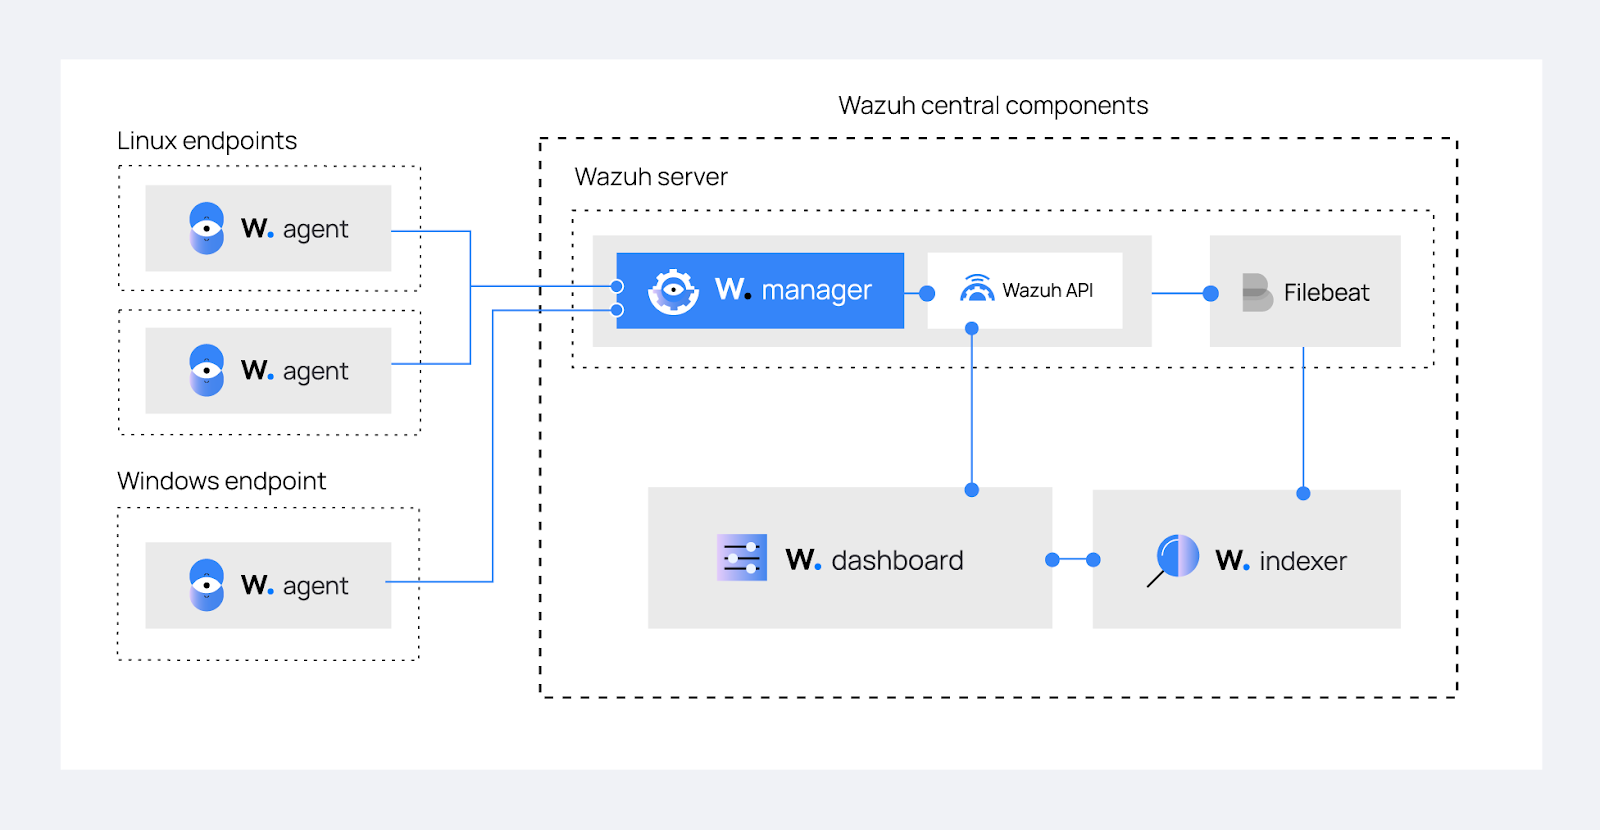
\includegraphics[width=16cm]{img/wazuh.png}
    \caption{\textit{Wazuh} įrankio komponentinė diagrama}
    \label{fig:wazuh}
\end{center}
\end{figure}

\textit{Wazuh} įrankis susideda iš kelių komponentų. \textit{Wazuh agent} yra komponentas, atsakingas už saugos įvykių registravimą ir žurnalinių įrašų stebėjimą klientinėje mašinoje. Šis komunikuoja su \textit{Wazuh manager} komponentu, kuris perduoda gautus duomenis iš klientinių mašinų indeksatoriui. Besinaudojant indeksatoriaus duomenimis \textit{Wazuh dashboard} vartotojo sąsajos komponentas atvaizduoja šiuos duomenis įvarus tipo diagramose ir pan.

\subsection{Programinės įrangos diegimas ir konfiguravimas}

Virtualios mašinos kuriamos naudojant \textit{Vagrant} įrankį, o pačios mašinos yra automatiškai sukonfiguruojamos naudojant \textit{Ansible} pjesėmis.

Naudojamos dvi virtualios mašinos, viena - \textit{Wazuh} serveris, kita - \textit{Wazuh} \textit{Ubuntu Linux} klientas. 

Diegimas vyksta keliais etapais. Pirmojo etapo metu yra sugeneruojami \textit{Wazuh} serverio sertifikatai, šie eksportuojami panaudojimui klientinėse mašinose. Šiuos sugeneravus, įdeigiami serverio komponentai, indeksatorius ir \textit{Wazuh dashboard}, kartu ir \textit{Wazuh manager} su \textit{Filebeat}.

Sudiegus serverį, galima pradėti konfiguruoti klientines mašinas, į jas diegiant \textit{Wazuh agent}. Visi veiksmai atliekami naudojantis \textit{Wazuh} suteikiamomis \textit{Ansible} pjesėmis ir rolėmis. 

Konfiguracija kuri sudiegiama naudojantis pateikiamomis pjesėmis yra tvarkinga ir atitinkati didžiąją dalį užduoties reikalavimų. \autoref{fig:log_aggregation} galime matyti jog sukonfiguruojami \textit{syslog} tipo žurnalinių įrašų nuskaitymas iš nurodytų failų. Šie įvykiai yra išsaugomi \textit{Wazuh} serveryje ir juos galima pamatyti \textit{Wazuh dashboard}. \autoref{fig:dir_checks} galime matyti saugos įvykių generavimo konfiguraciją, šiose direktorijose atlikti veikmai sugeneruotu įvykius, kurie būtų patalpinti serveryje.

\textit{Wazuh} nesuteikia funkcionalumo automatiškai ištrinti žuranlinius įrašus ar įvykius, tačiau tai galima atlikti naudojant \textit{cronjob} funkcionalumą.

\begin{figure}[H]
    \begin{center}
        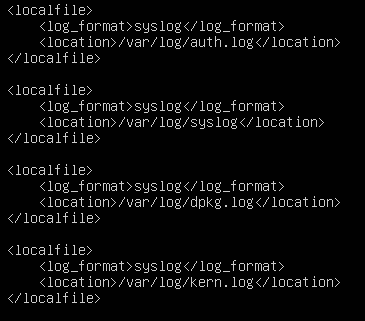
\includegraphics[width=10cm]{img/log_aggregation.png}
        \caption{Žurnalinių įrašų agregacijos konfiguracija}
        \label{fig:log_aggregation}
    \end{center}
\end{figure}


\begin{figure}[H]
    \begin{center}
        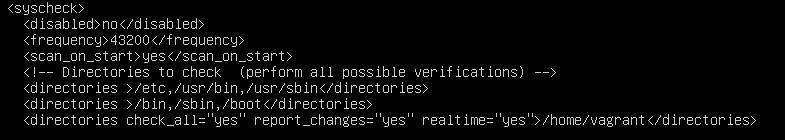
\includegraphics[width=16cm]{img/dir_checks.png}
        \caption{Saugos įvykių nurodytose direktorijose agregacijos konfiguracija}
        \label{fig:dir_checks}
    \end{center}
\end{figure}

Sistema taip pat atlieka didelį kiekį įvairaus tipo patikrų, kaip \textit{CIS} ar pažeidžiamumų patikros. 


\begin{figure}[H]
    \begin{center}
        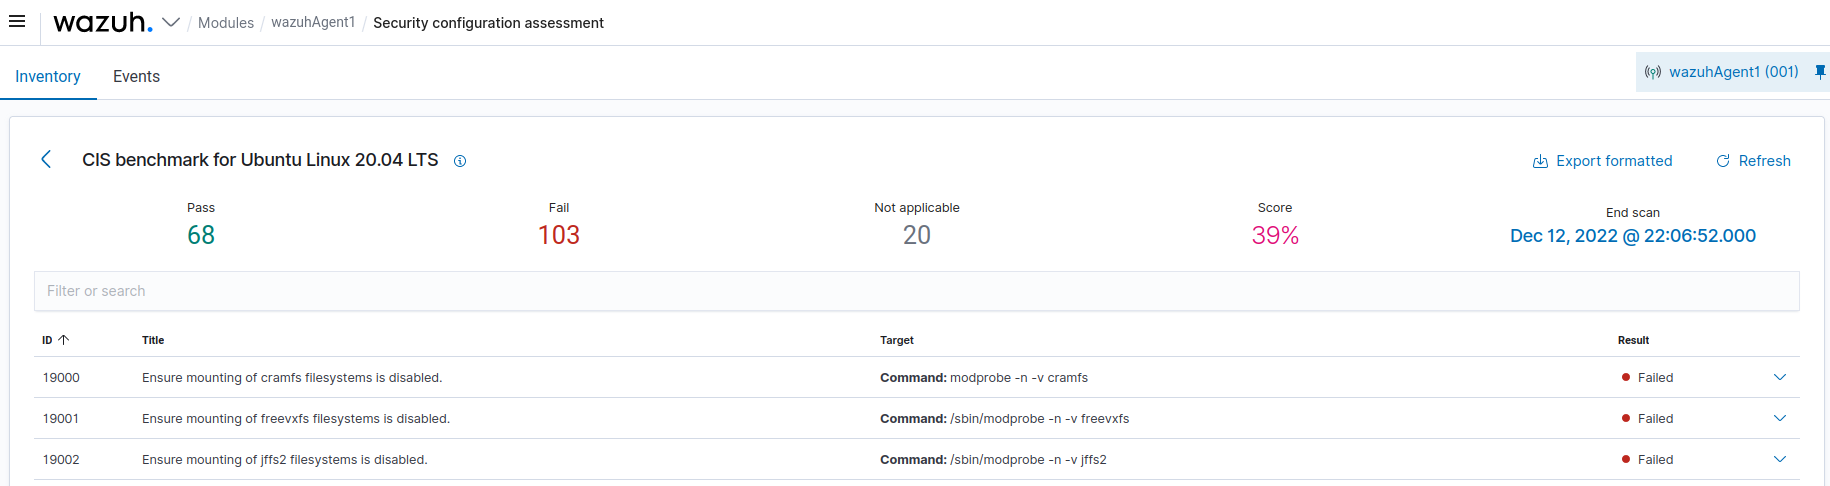
\includegraphics[width=16cm]{img/security_assesments.png}
        \caption{\textit{CIS} patikros rezultatai \textit{wazuhAgent1} agentui}
        \label{fig:security_assesments}
    \end{center}
\end{figure}

\subsection{Užduoties reikalavimų įgyvendinimas}

Įdiegta \textit{Wazuh} SIEM sistema nuskaito žurnalinius įrašus, generuoja saugumo įvykius ir pranešimus. Taip įgyvendinami pirmi trys užduoties reikalavimai. Penktasis reikalavimas gali būti įgyvendinamas naudojant \textit{crontab} funkcionalumą serveryje.

\VTDocumentEnd